\section{The Renormalization Group}
\subsection{When is perturbation theory any good? - A classification of couplings}
We revisit the last comment from our previous lecture. We had noticed that couplings are (typically) dimensionful, and hence it is not meaningful to say they are ``small''. E.g. $[\lambda_{\phi^3}] = \frac{D-6}{2}$. So, really the expansion parameter is not the coupling, but the coupling times some energy scale; $\lambda_{\phi^3}/E^{\frac{6-D}{2}} \ll 1$. This depends on what observable we study, and influences where perturbation theory works.

In the example that we computed, if we set $m = 0$ then:
\begin{equation}
    G_{\text{int}}(p) = \frac{-i}{p^2}\left(1 + C\frac{\lambda^2}{(p^2)^{[\lambda]}} + \ldots\right)
\end{equation}
The energy scale is set by $p^2$, i.e. $E \sim \sqrt{p^2}$. Depending on the dimensions our notion of ``small'' changes.

\emph{Relevant couplings} are those with $[\lambda] > 0$. Then, the perturbation theory is controlled at high energies (compared to the coupling). Theories with only relevant interactions/couplings are called \emph{asymptotically free} (at high energies, they become free). They have the property of being \emph{UV-complete}, because in principle they provide a complete microscopic definition of a theory. They are also called \emph{renormalizable} (though this is older, and arguably questionable, terminology).

\emph{Irrelevant couplings} are those with $[\lambda] < 0$. Then, perturbation theory is controlled at low energies (compared to the coupling). QFTs with irrelevant couplings are known as ``effective field theories'' - they cannot be theories of everything (there is a more complete theory at higher energy/shorter length scales, and the UV is unknown) but still can be massively useful in making predictions.

\begin{center}
    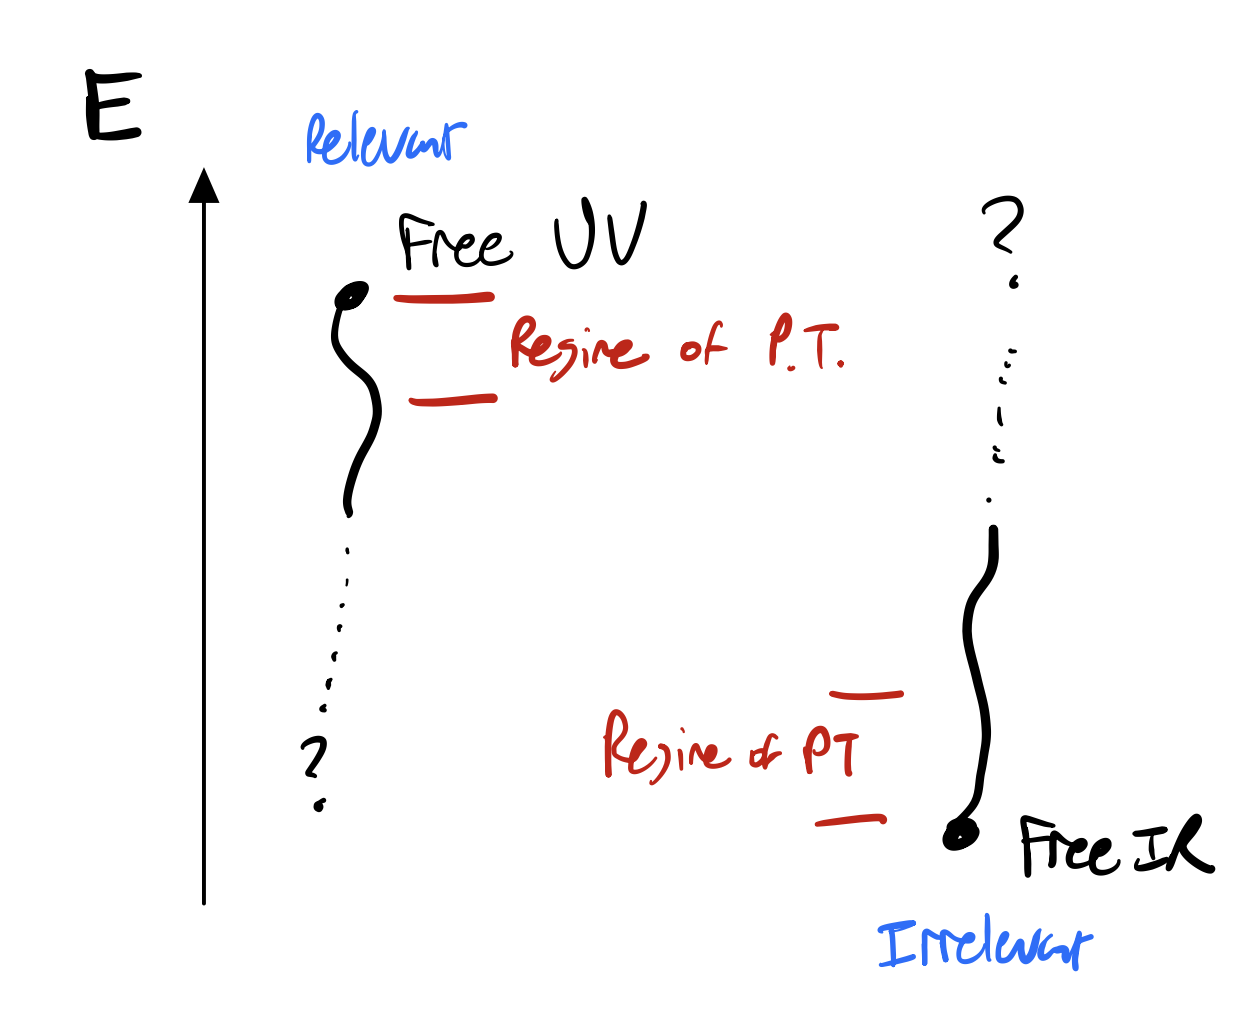
\includegraphics[scale=0.4]{Lectures/Figures/lec14-ptvalidity.png}
\end{center}

\emph{Marginal couplings} are those with $[\lambda] = 0$. This would be the $D = 6$ case for the $\phi^3$ theory. This seems like a fine-tuned example, but actually applies to many interesting theories, e.g. QED. In this case, if we compute the loop corrections, they do not give power law corrections to the momenta, but rather (dimensionless) logarithms. E.g. looking at the non-analytic part of the correction in $\phi^3$ theory:
\begin{equation}
    G_{\text{int}}(p) = \frac{-i}{p^2}\left(1 + \lambda^2 \log \frac{p}{\Lambda} + \ldots\right)
\end{equation}
Now the issue here is that the perturbation theory seems to break down when both $p \to 0$ and $p \to \infty$. Said another way, we see a breakdown both at high/low energies, or both in the UV and the IR. So is PT actually useless here? Actually, slightly more careful analysis will save the day, and will show that marginal couplings also become large in the UV \emph{or} the IR, not both. We can thus consider such couplings as either marginally relevant or irrelevant. However, we have to go beyond simple dimensional analysis to figure this out. It will be theory dependent. The machinery that will allow us to tackle this is the \emph{renormalization group}.

\subsection{Motivating/Introducing the Renormalization Group}
Pragmatically, RG will allow us to ``resum the logarithms'' for theories with marginal couplings, recovering controlled perturbative predictions. But, it has deep consequences beyond this. For one, it connects particle physics with statistical mechanics. Additionally, it introduces the possibility of special quantum field theories, known as conformal field theories (CFTs) which are fixed points of the renormalization group. RG asks ``what happens as we change scales in a theory?'' and CFTs are special theories that are scale invariant. Originally when CFTs were introduced, they were originally thought as special theories with no experimental consequence (as our world is full of scale-dependent thing) but now they are seen in a different light; they are seen as special corners of theories which can make predictions via addition of different couplings. They are very powerful, allowing for non-perturbative approaches to QFT. They also give a way to define string theory.

RG is arguably one of the biggest developments of theoretical physics in the last century\footnote{Was partly developed in Chicago! Invented by Wilson, Kadanoff\ldots}. Conceptually, we want to ask the question of ``how does a theory change under coarse graining''? We may have some microscopic description of a system, and want to coarse grain. Under this coarse graining, the original microscopic action $S$ will map to an effective action $S_{\text{eff}}$ with slightly different effective couplings. 

\begin{center}
    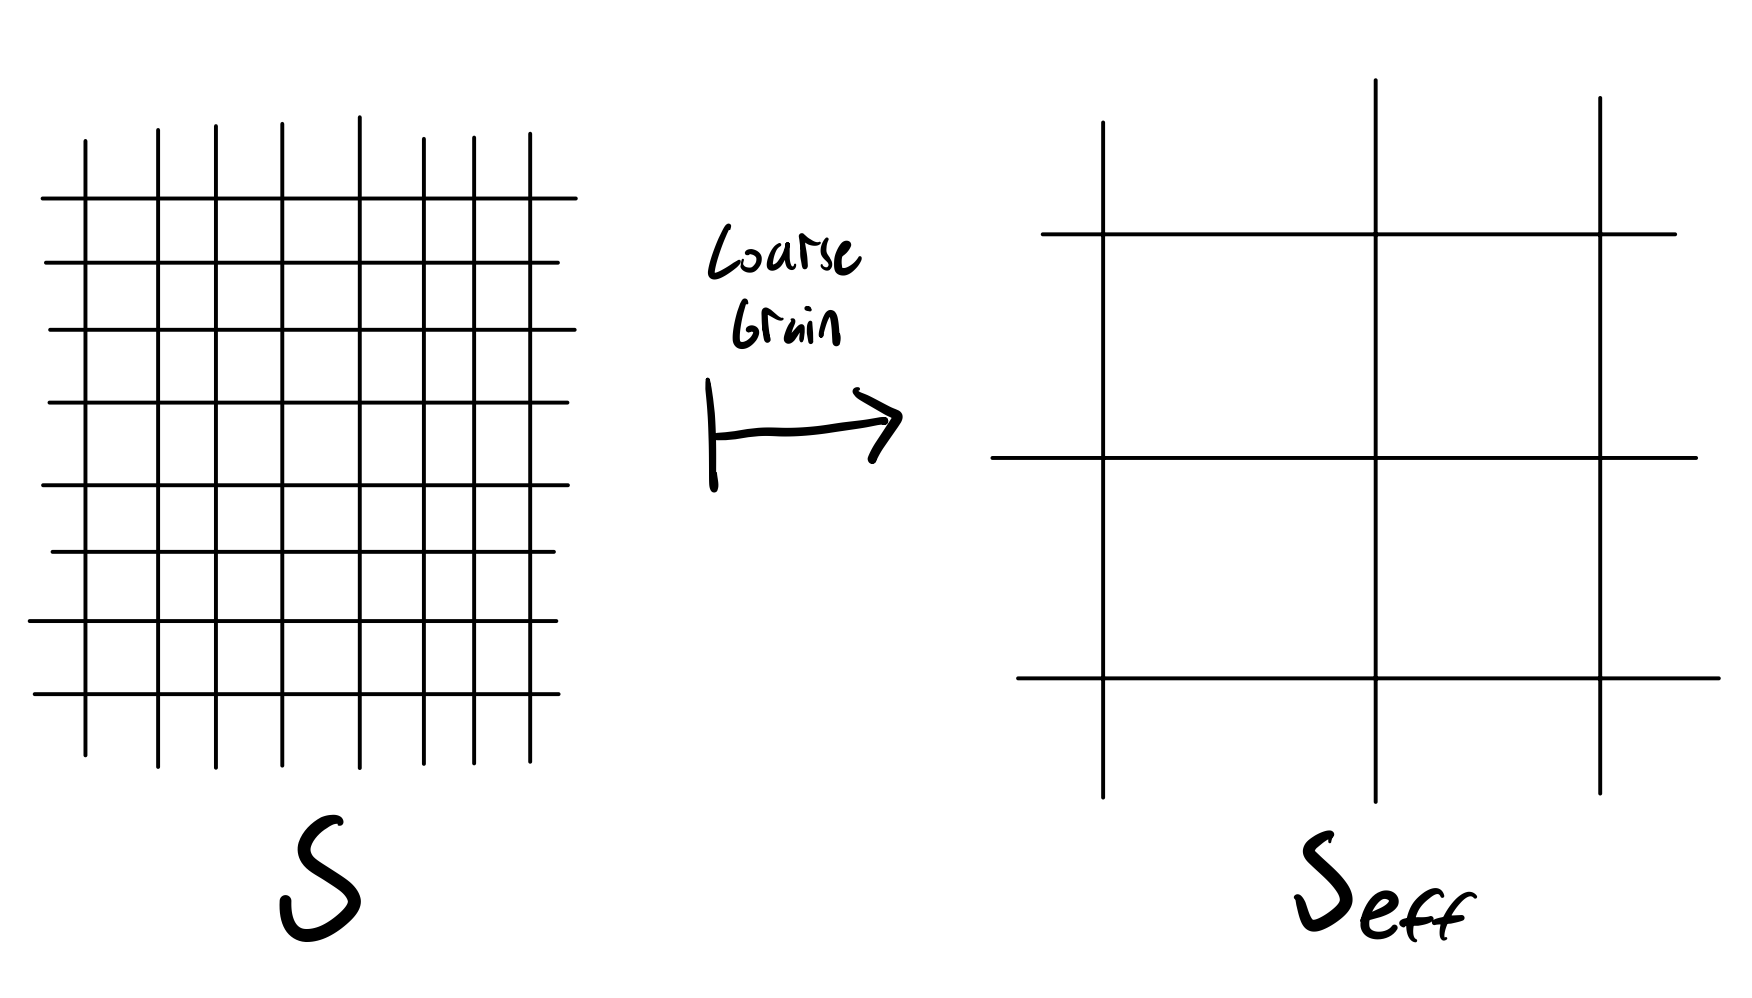
\includegraphics[scale=0.3]{Lectures/Figures/lec14-coarsegrain.png}
\end{center}

Couplings that \emph{grow} are relevant, and those that shrink are irrelevant. This coarse-graining procedure is what is called a renormalization group flow. Pictorially, we imagine that there are flows in the space of theories, where $S$ flows to $S_{\text{eff}}$.

\begin{center}
    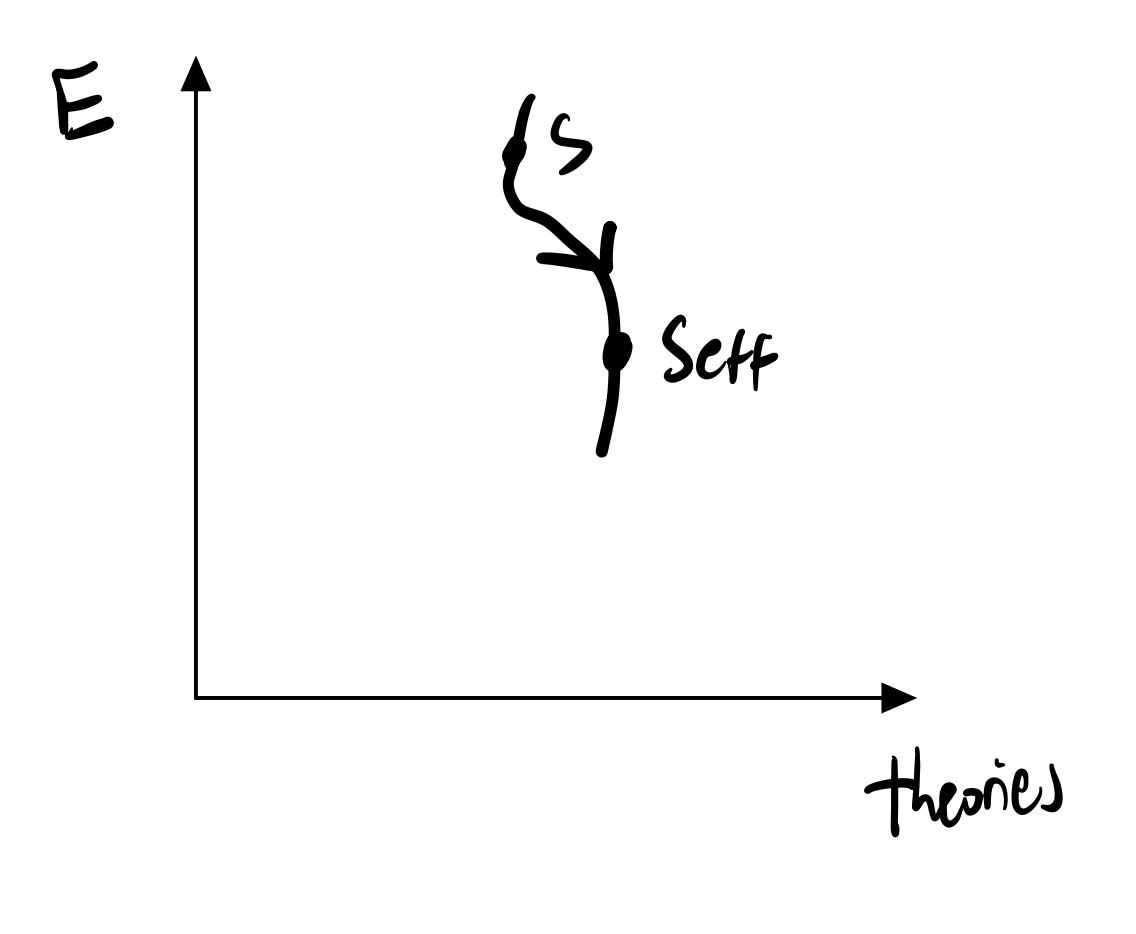
\includegraphics[scale=0.35]{Lectures/Figures/lec14-rgflow.png}
\end{center}

In QFT there is a very elegant way to implement this using the path integral, which we will now begin to explore. A useful reference for this part of the course is Chapter 12 of Peskin and Schroeder.

\subsection{Case Study - Looking at $\phi^4$ theory}
Srednicki uses $\phi^3$, where the interesting questions are in $D = 6$... so let's instead look at $\phi^4$ theory, where there are interesting things happening in $D = 4$ (else Luca would feel bad if this was your only QFT course and you only got to study 6 spacetime dimensions, which is beyond our everyday experience). Our action takes the form:
\begin{equation}
    S = \int d^Dx \frac{1}{2}(\p_\mu \phi)^2 + \frac{1}{2}m^2\phi^2 + \frac{1}{4!}\lambda \phi^4
\end{equation}
Doing dimensional analysis, we have (for the action to be dimensionless):
\begin{equation}
    [\phi] = \frac{D-2}{2}, [m] = 1
\end{equation}
and then looking at the dimension of $\lambda$:
\begin{equation}
    1 \sim \frac{S_{\text{int}}}{S_{\text{m}}} \sim \frac{\lambda\phi^4}{m^2} \sim \lambda E^{D-4} \implies [\lambda] = 4-D
\end{equation}
For $D < 4$, the coupling is relevant (going to higher energies we get more perturbative control). For $D > 4$ it is irrelevant (going to lower energies we get more perturbative control). For $D = 6$ the coupling is marginal, and we don't know (yet) where we need to go to get control over our theory - we need to do more work.

The way we implement RG in QFT using the path integral is quite nice. What we can do is integrate out (path integrate) all fields with momentum beyond/above some value (i.e. energies above a certain scale/below some length scale), and we will see how the couplings flow when we do this. To simplify, let us Wick rotate from the start, $t \to it_E$:
\begin{equation}
    e^{iS} \to e^{-S_E}
\end{equation}
with:
\begin{equation}
    S_E = \int d^Dx \frac{1}{2}(\nabla \phi)^2 + \frac{1}{2}m^2 \phi^2 + \frac{1}{4!}\lambda\phi^4
\end{equation}
now, its quite clear that we are doing statistical mechanics, with $S_E$ taking the role of $\beta H$. Instead of looking at $3+1$ dimensions (3 spatial, 1 time), the problem is now in 4 spatial dimensions. Consider the path integral:

\begin{equation}
    Z = \int \prod_x d\phi(x)e^{-S_E} = \int \prod_k d\phi_k e^{-S_E(\phi_k)}
\end{equation}
We now consider a slightly different object; a path integral where all modes with $k > \Lambda$ have already been integrated out:
\begin{equation}
    Z_\Lambda = \int \prod_{k < \Lambda}d\phi_k e^{-S_E}
\end{equation}
In the coarse graining step, we then integrate out all $\phi_k$ with $b\Lambda < \abs{k} < \Lambda$, with $0 < b < 1$ and $1 - b \ll 1$.

\begin{center}
    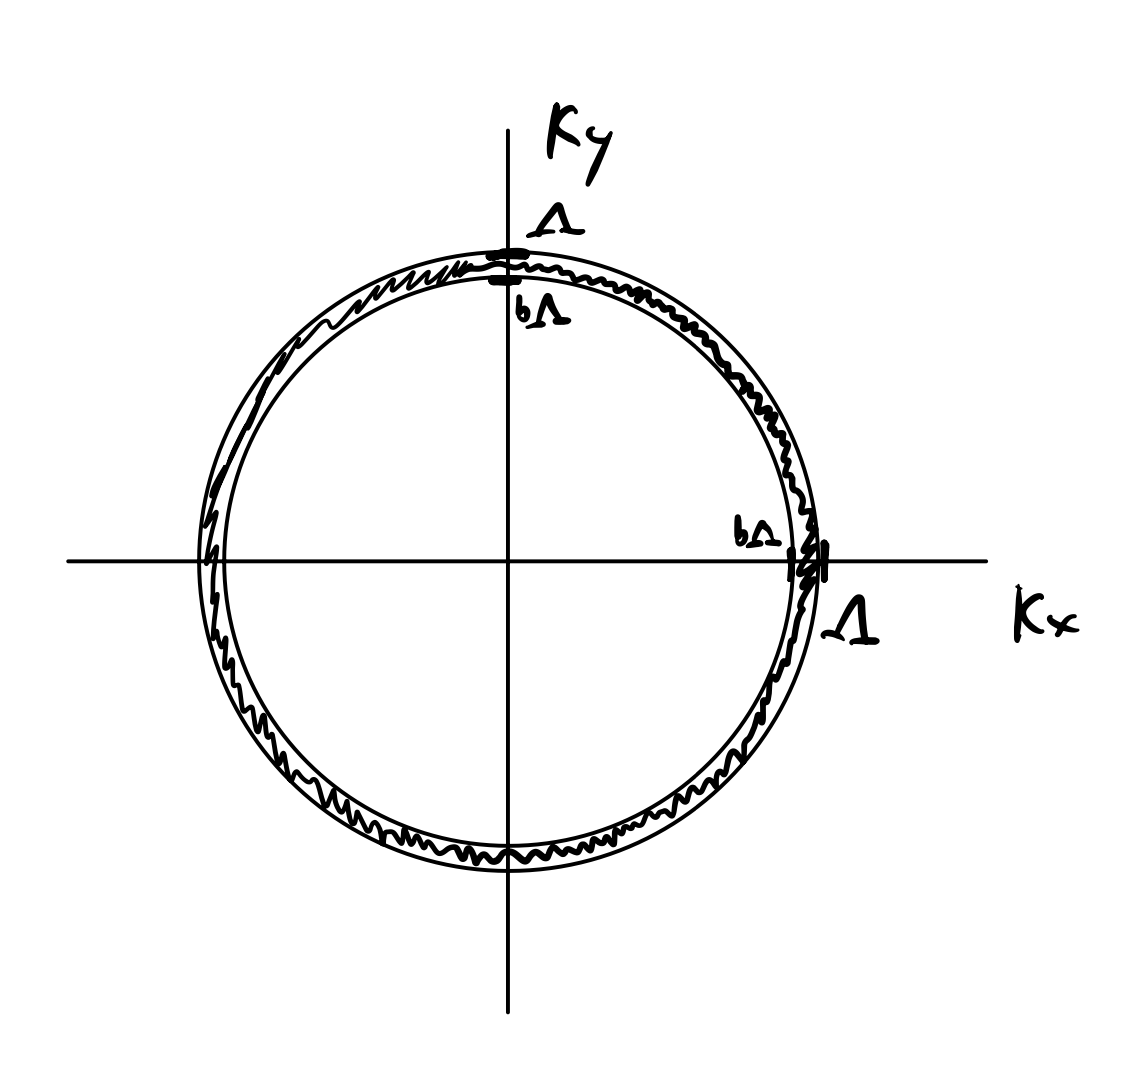
\includegraphics[scale=0.35]{Lectures/Figures/lec14-momentumshell.png}
\end{center}
We then compare to $Z_{\Lambda}$.

\subsection{Free-theory warm-up}
We consider:
\begin{equation}
    S_E = \int d^4x \frac{1}{2}(\nabla \phi)^2 + \frac{1}{2}m^2\phi^2 = \int_{k < \Lambda} \frac{d^4k}{(2\pi)^4}\frac{1}{2}(k^2 + m^2)\phi_{k}\phi_{-k}
\end{equation}
where note that in the free theories the momentum modes do not couple. We've already integrated out modes higher than $\Lambda$. Now, we split this integral:
\begin{equation}
    S_E = \int_{k < b\Lambda}\frac{1}{2}(k^2 + m^2)\phi_k\phi_{-k} + \int_{b\Lambda < k < \Lambda}\frac{1}{2}(k^2 + m^2)\phi'_{k}\phi'_{-k}
\end{equation}
where we use $\phi_k$ to denote modes with $k < b\Lambda$ and $\phi_k'$ to denote modes with $b\Lambda < k < \Lambda$. We then have:
\begin{equation}
    \begin{split}
        Z_\Lambda &= \int \prod_{k < b\Lambda}d\phi_k \int \prod_{b \Lambda < k < \Lambda} d\phi_k' e^{-S}
        \\ &= \int \prod_{k < b\Lambda}d\phi_k e^{-\frac{1}{2}\int_{k < b\Lambda}(k^2 + m^2 \phi_k \phi_{-k})} \int \prod_{b\Lambda < k < \Lambda}d\phi_k' e^{-\frac{1}{2}\int_{b\Lambda < k < \Lambda}(k^2 + m^2)\phi_k'\phi_{-k}'}
    \end{split}
\end{equation}
The integral over the $\phi_k'$s just gives a number independent of $\phi$ (call it $C$) and we are left with just the path integral over the low energy modes:
\begin{equation}
    Z_\Lambda = C\int \prod_{k < b\Lambda}d\phi_k d\phi_k e^{-\frac{1}{2}\int_{k < b\Lambda}\frac{1}{2}(k^2 + m^2)\phi_k \phi_{-k}}
\end{equation}
Now, we want to compare this to what we started with. In order for the range of momenta to match, we substitute $\tilde{k} = \frac{k}{b} < \Lambda$.
\begin{equation}
    Z_\Lambda = \int \prod_{\tilde{k} < \Lambda}d\phi_{\tilde{k}} e^{-\int_{\tilde{k} < \Lambda}\frac{1}{2}b^4(b^2 \tilde{k}^2 + m^2)\phi_{\tilde{k}}\phi_{-\tilde{k}}}
\end{equation}
Now rescale the field $\tilde{\phi} = b^3\phi$ to have a canonical kinetic term:
\begin{equation}
    Z_{\Lambda} = \int \prod_{\tilde{k} < \Lambda}d\phi_{\tilde{k}} e^{-\int_{\tilde{k} < \Lambda}\frac{1}{2}(\tilde{k}^2 + \frac{m^2}{b^2})\phi_{\tilde{k}}\phi_{-\tilde{k}}}
\end{equation}
We see that the effective $m^2$ has grown, with $m^2 \to \frac{m^2}{b^2}$. This is a very complicated way to make a very obvious statement. Recall the propagator of the free scalar is:
\begin{equation}
    G(k) = \frac{1}{k^2 + m^2}
\end{equation}
So all this is saying is that as we decrease the energy $k$, the effect of the mass $m$ grows. Thus, we would say that $m^2$ is \emph{relevant}, because it matters more at low energies/under coarse graining. This is the same thing that we would have obtained by doing dimensional analysis.

Now we have all the ingredients we need to study the renormalization of a $\phi^4$ interacting theory.

\subsection{Back to renormalization of $\phi^4$}
We return to:
\begin{equation}
    S = \int d^4x \frac{1}{2}(\nabla \phi)^2 + \frac{1}{2}m^2 \phi^2 + \frac{1}{4!}\lambda\phi^4
\end{equation}
When we fourier transform the $\phi^4$ term, we get something of the form:
\begin{equation}
    \int_{k_1k_2k_3}\phi_{k_1}\phi_{k_2}\phi_{k_3}\phi_{-k_1-k_2-k_3}
\end{equation}
which is more subtle than what we had before, the RG mixes the high and low energy modes. Suppose we split into $\phi, \phi'$:
\begin{equation}
    S[\phi + \phi'] = \int d^4x \frac{1}{2}(\p(\phi + \phi'))^2 + \frac{1}{2}m^2(\phi + \phi')^2 + \frac{\lambda}{4!}(\phi + \phi')^4
\end{equation}
So looking at the partition function:
\begin{equation}
    Z = \int D\phi e^{-S(\phi)}\int D\phi' \exp(-\int \frac{1}{2}(\p\phi')^2 + \frac{1}{2}m^2\phi'^2 + \frac{\lambda}{4!}(\phi'^4 + 4\phi'^3\phi + 6\phi'^2\phi^2 + 4\phi'\phi^3))
\end{equation}
we see that the last term indeed mixes the high and low energy modes. Let's expand:
\begin{equation}
    Z = \int D\Phi e^{-S(\phi)}\int D\phi' e^{-S(\phi')} [1 - \frac{\lambda}{4!}\int d^4x (4\phi'^3\phi + 6\phi'^2\phi^2 + 4\phi'\phi^3) + \ldots]
\end{equation}
We can view the $\phi$ in the $\phi'$ integral as an external source:
\begin{equation}
    Z = \int D\Phi e^{-S(\phi)}\left(1 - \frac{\lambda}{4!}\int d^4x 4\phi(x)\avg{\phi'^3(x)} + 6\phi^2(x)\avg{\phi'^2(x)} + 4\phi^3(x)\avg{\phi'(x)}\right)
\end{equation}
now, by the $\mathbb{Z}_2$ symmetry of the theory the one and three point functions vanish, so we are left with:
\begin{equation}
    Z = \int D\Phi e^{-S(\phi)}\left(1 - \frac{\lambda}{4!}\int d^4x + 6\phi^2(x)\avg{\phi'^2(x)}\right)
\end{equation}
Diagramatically, the contribution of this term looks like:

\begin{center}
    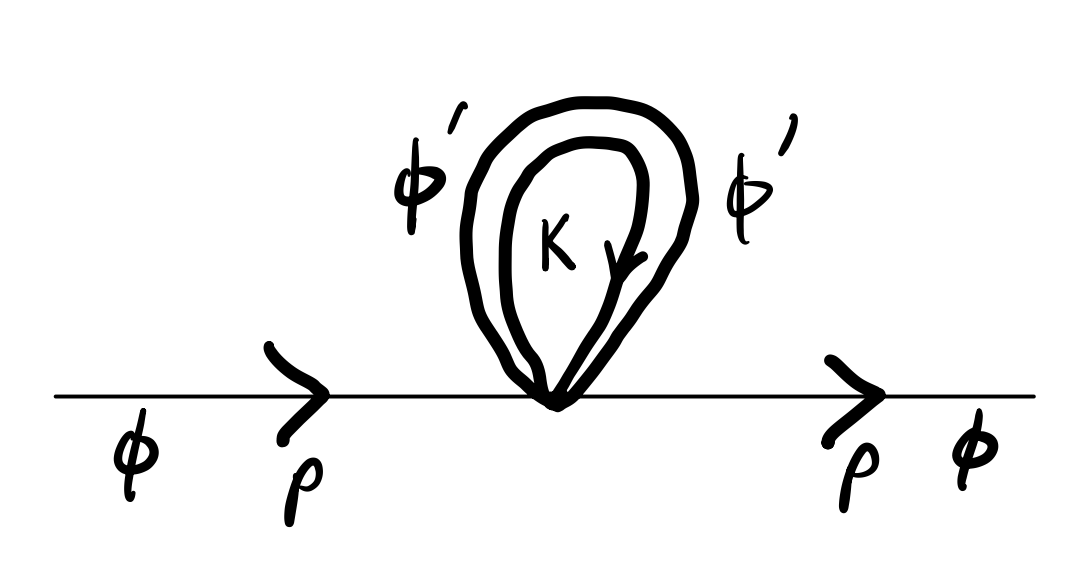
\includegraphics[scale=0.35]{Lectures/Figures/lec14-massrenorm.png}
\end{center}

Let's compute the two point function. This is similar to the free field two-point function we know, but we only integrate over the modes between $b\Lambda$ and $\Lambda$:
\begin{equation}
    \avg{\hat{\phi}'^2(x)} = \avg{\phi'(x)\phi'(x)} = \int_{b\Lambda < k < \Lambda}\frac{d^4k}{(2\pi)^4}\frac{1}{k^2 + m^2} = \frac{2\pi^2}{(2\pi)^4}\int_{b\Lambda}^\Lambda dk \frac{k^3}{k^2 + m^2}
\end{equation}
Now if we assume that $m \gg \Lambda$, then since $k \sim \Lambda$ we have:
\begin{equation}
    \avg{\hat{\phi}'^2(x)} \approx \frac{1}{8\pi^2}\int_{b\Lambda}^\Lambda dkk = \frac{1}{16\pi^2}(\Lambda^2 - (b\Lambda)^2) = \frac{\Lambda^2}{(4\pi)^2}(1 - b^2).
\end{equation}
Thus, we see that the effect of the interaction at this order is to add a term in the path integral for the low energy modes:
\begin{equation}
    Z = \int D\phi e^{-S(\phi)}\left(1 - \frac{\lambda}{2}\int d^4x \phi^2(x)\frac{\Lambda^2}{(4\pi)^2}(1 - b^2) + \ldots \right)
\end{equation}
We reinterpret this small quantity as an exponential:
\begin{equation}
    \exp(-\delta S), \quad \delta S = \frac{1}{2}\int d^4x \frac{\lambda \Lambda^2}{(4\pi)^2}(1 - b)^2\phi^2(x)
\end{equation}
so what did this interaction do? It renormalized the mass by the above amount, so the effective action is now:
\begin{equation}
    S_{\text{eff}} = \frac{1}{2}\int (\nabla \phi)^2 + (m^2 + \delta m^2)\phi^2
\end{equation}
where the mass gets ``dressed'' by the high energy modes. Next week, we will look at higher orders, and we will see that the interactions also renormalize themselves!! (We will then see the fate of $\lambda$!) For example at $O(\lambda^2) $, we will have the contribution:

\begin{center}
    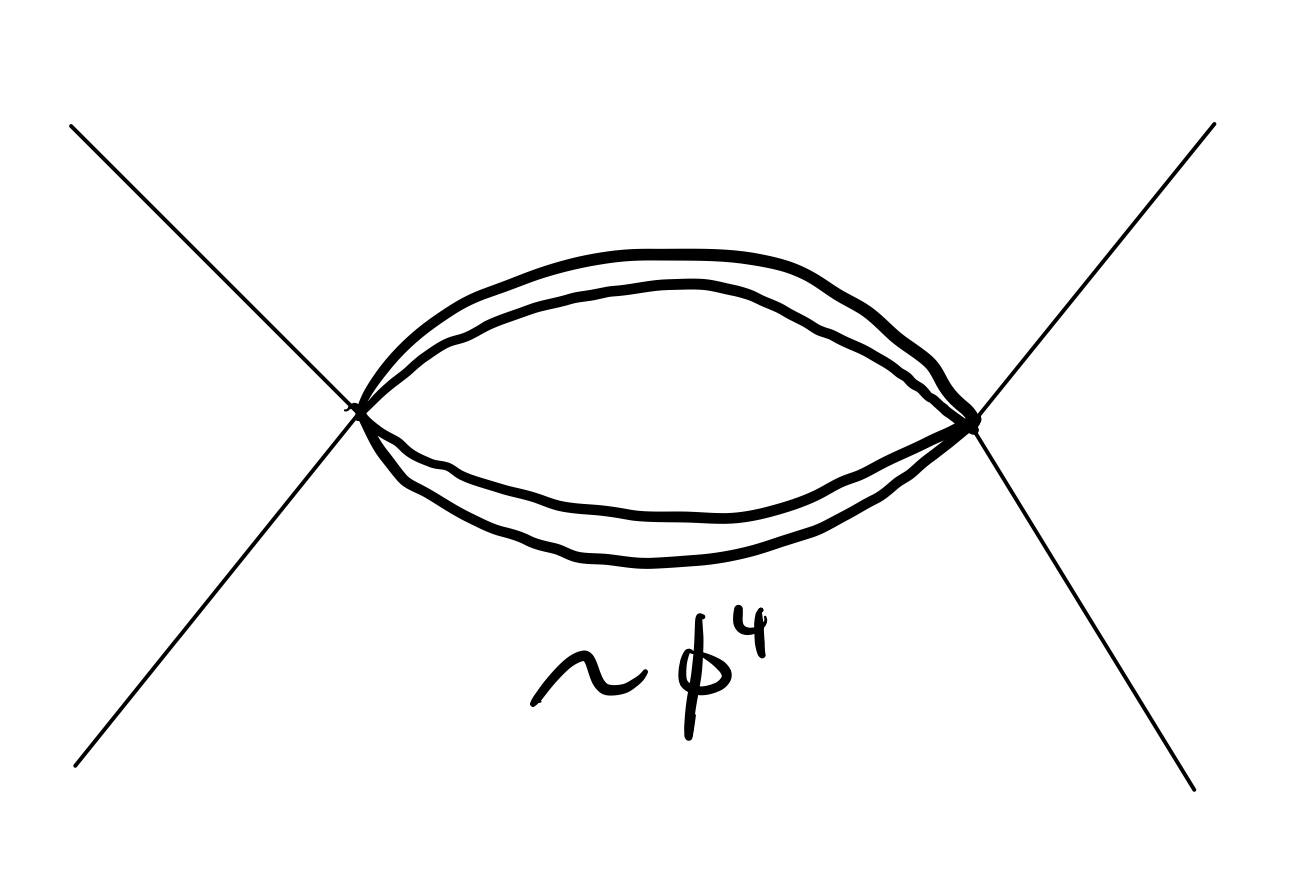
\includegraphics[scale=0.35]{Lectures/Figures/lec14-interactionrenorm.png}
\end{center}



